\documentclass{beamer}

\newcommand{\lesson}{Inheritance, Part 1 of 2}

\author[Chris Simpkins] 
{Christopher Simpkins \\\texttt{chris.simpkins@gatech.edu}}
\institute[Georgia Tech] % (optional, but mostly needed)

\date{}


\newcommand{\course}{Introduction to Object-Oriented Programming}
\subject{\course}
\title[\lesson]{\course}
\subtitle{\lesson}

\author[CS 1331]
{Christopher Simpkins \\\texttt{chris.simpkins@gatech.edu}}
\institute[Georgia Tech]

\date[]{}

\newcommand{\link}[2]{\href{#1}{\textcolor{blue}{\underline{#2}}}}
\newcommand{\code}{http://www.cs1331.org/code}

\usepackage{colortbl}

% If you have a file called "university-logo-filename.xxx", where xxx
% is a graphic format that can be processed by latex or pdflatex,
% resp., then you can add a logo as follows:

% \pgfdeclareimage[width=0.6in]{coc-logo}{cc_2012_logo}
% \logo{\pgfuseimage{coc-logo}}

\mode<presentation>
{
  \usetheme{Berlin}
  \useoutertheme{infolines}

  % or ...

 \setbeamercovered{transparent}
  % or whatever (possibly just delete it)
}

\usepackage{tikz}
% Optional PGF libraries
\usepackage{pgflibraryarrows}
\usepackage{pgflibrarysnakes}
\usepackage{pgfplots}
\usepackage{fancybox}
\usepackage{listings}
\usepackage{hyperref}
\hypersetup{colorlinks=true,urlcolor=blue}
\usepackage[english]{babel}
% or whatever

\usepackage[latin1]{inputenc}
% or whatever

\usepackage{times}
\usepackage[T1]{fontenc}
% Or whatever. Note that the encoding and the font should match. If T1
% does not look nice, try deleting the line with the fontenc.


\usepackage{listings}

% "define" Scala
\lstdefinelanguage{scala}{
  morekeywords={abstract,case,catch,class,def,%
    do,else,extends,false,final,finally,%
    for,if,implicit,import,match,mixin,%
    new,null,object,override,package,%
    private,protected,requires,return,sealed,%
    super,this,throw,trait,true,try,%
    type,val,var,while,with,yield},
  otherkeywords={=>,<-,<\%,<:,>:,\#,@},
  sensitive=true,
  morecomment=[l]{//},
  morecomment=[n]{/*}{*/},
  morestring=[b]",
  morestring=[b]',
  morestring=[b]""",
}

\usepackage{color}
\definecolor{dkgreen}{rgb}{0,0.6,0}
\definecolor{gray}{rgb}{0.5,0.5,0.5}
\definecolor{mauve}{rgb}{0.58,0,0.82}

% Default settings for code listings
\lstset{frame=tb,
  language=scala,
  aboveskip=2mm,
  belowskip=2mm,
  showstringspaces=false,
  columns=flexible,
  basicstyle={\scriptsize\ttfamily},
  numbers=none,
  numberstyle=\tiny\color{gray},
  keywordstyle=\color{blue},
  commentstyle=\color{dkgreen},
  stringstyle=\color{mauve},
  frame=single,
  breaklines=true,
  breakatwhitespace=true,
  keepspaces=true
  %tabsize=3
}


% \beamerdefaultoverlayspecification{<+->}


\begin{document}

\begin{frame}
  \titlepage
\end{frame}

%------------------------------------------------------------------------
\begin{frame}[fragile]{Programming in the Large}


Software is complex.  Three ways we deal with complexity:
\begin{itemize}
\item Abstraction - boiling a concept down to its essential elements, ignoring irrelevant details
\item Decomposition - decompose system into packages, classes, functions
\item Reuse - reuse library function in many diferent places
\end{itemize}
\vspace{.1in}
Today we introduce another kind of resuse: inheritance

\end{frame}
%------------------------------------------------------------------------

%------------------------------------------------------------------------
\begin{frame}[fragile]{What is inheritance?}

\begin{center}

\includegraphics[height=2.5in]{money_Inheritance.jpg}\footnote{Source: http://talentenbank.com/can-you-really-make-inheritance-into-a-good-financial-move-in-the-long-run}
\end{center}

\end{frame}
%------------------------------------------------------------------------

%------------------------------------------------------------------------
\begin{frame}[fragile]{What is inheritance?}


More like genetics ...
\begin{center}
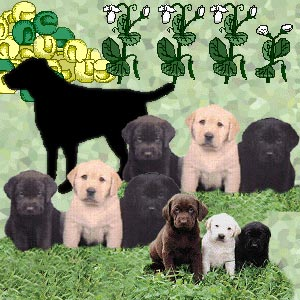
\includegraphics[height=2in]{puppy-inheritance.jpg}\footnote{Source: http://www.dnaftb.org/5/}\\
\end{center}
... but a programming concept that, like so much in CS, borrows a term from another field to leverage our intuition.

\end{frame}
%------------------------------------------------------------------------

%------------------------------------------------------------------------
\begin{frame}[fragile]{Inheritance}


Inheritance:  deriving one class from another class.
\begin{lstlisting}[language=Java]
public class Employee { ... }
public class HourlyEmployee extends Employee { ... }
public class SalariedEmployee extends Employee { ... }
\end{lstlisting}

\begin{itemize}
\item {\tt Employee} is the {\it base class} or {\it superclass}
\item {\tt HourlyEmployee} and {\tt SalariedEmployee} are {\it derived classes} or {\it subclasses}
\item Subclasses {\it inherit} the interface and implementation of their superclass(es)
\item {\tt extends} is the Java syntax for inheriting from another class
\end{itemize}

Important idea to plant in your head now: subclassing is about concept reuse not merely implementation reuse.  For example, {\tt HourlyEmployee} {\it is-a} {\tt Employee} conceptually.  

\end{frame}
%------------------------------------------------------------------------

%------------------------------------------------------------------------
\begin{frame}[fragile]{Superclasses}

\vspace{-.05in}
Consider the superclass \href{\code/employee/Employee1.java}{Employee1}:\footnote{Note that we'll number the versions of our Employee classes like we did with Card.}
\vspace{-.05in}
\begin{lstlisting}[language=Java]
public class Employee1 {
    private String name;
    private Date hireDate;

    public Employee1(String aName, Date aHireDate) {
        disallowNullArguments(aName, aHireDate);
        name = aName;
        hireDate = aHireDate;
    }
    public String getName() {
        return name;
    }
    public Date getHireDate() {
        return hireDate;
    } // and toString(), etc. ...
}
\end{lstlisting}
\vspace{-.05in}
{\tt Employee} defines the basic information needed to define any employee.

\end{frame}
%------------------------------------------------------------------------

%------------------------------------------------------------------------
\begin{frame}[fragile]{Subclasses}


The {\tt extends} clause names the direct superclass of the current class (\href{http://docs.oracle.com/javase/specs/jls/se7/html/jls-8.html#jls-8.1.4)}{JLS \S 8.1.4}).

Here is a subclass of {\tt Employee1},  \link{\code/employee/HourlyEmployee1.java}{HourlyEmployee1}:
\begin{lstlisting}[language=Java]
public class HourlyEmployee extends Employee {

    public HourlyEmployee(String aName, Date aHireDate) {
        super(aName, aHireDate);
    }
}
\end{lstlisting}

\begin{itemize}
\item {\tt HourlyEmployee} inherits all the members of {\tt Employee}
\item {\tt HourlyEmployee} can't access private members of {\tt Employee} directly
\item The {\tt super} call in the constructor calls {\tt Employee}'s constructor to initialize {\tt HourlyEmployee} instances
\end{itemize}
The {\tt HourlyEmployee} concept extends the {\tt Employee} concept.

\end{frame}
%------------------------------------------------------------------------

%------------------------------------------------------------------------
\begin{frame}[fragile]{{\tt super} Subtleties}


\begin{itemize}
\item If present, an explicit {\tt super} call must be the first statement in a constructor.
\item If an explicit {\tt super} call is not present and the superclass has a no-arg constructor, {\tt super()} will implicitly be the first statement in any constructor
\item If there is no no-arg constructor in a superclass (for example, if the superclass defines other constructors without explicitly defining a no-arg constructor), then subclass constructors must explicitly include a {\tt super} call.
\end{itemize}
Together, these rules enforce an ``inside-out'' construction order for objects: the highest superclass piece of an object is initialzed first, followed by the second highest, and so on.

\end{frame}
%------------------------------------------------------------------------

%------------------------------------------------------------------------
\begin{frame}[fragile]{Subclass Constructors}


Recall our definitions of {\tt Employee1} and {\tt HourlyEmployee1}.
\begin{lstlisting}[language=Java]
public class Employee1 {
    // The only constructor in Employee
    public Employee1(String aName, Date aHireDate) {
        disallowNullArguments(aName, aHireDate);
        name = aName;
        hireDate = aHireDate;
    }
    // ...
}
\end{lstlisting}

\begin{lstlisting}[language=Java]
public class HourlyEmployee1 extends Employee1 {

    public HourlyEmployee1(String aName, Date aHireDate) {
        super(aName, aHireDate);
    }
}
\end{lstlisting}

Would {\tt HourlyEmployee1.java} compile if we left off the constructor definition?

\end{frame}
%------------------------------------------------------------------------


%------------------------------------------------------------------------
\begin{frame}[fragile]{Inherited Members}


Given our previous definitions of {\tt Employee1} and {\tt HourlyEmployee1}, we can write code like this (from \link{\code/employee/EmployeeDemo1.java}{EmployeeDemo1}):
\begin{lstlisting}[language=Java]
DateFormat df = DateFormat.getDateInstance();
HourlyEmployee eva = new HourlyEmployee("Eva L. Uator",
                                        df.parse("February 18, 2013"));
System.out.println(eva.getName() + " was hired on " 
                   + eva.getHireDate());
\end{lstlisting}
Note that
\begin{itemize}
\item we didn't have to define {\tt getName} and {\tt getHireDate} in {\tt HourlyEmployee}
\item our current implementation of {\tt HourlyEmployee} doesn't add anything to {\tt Employee}
\end{itemize}


\end{frame}
%------------------------------------------------------------------------

%------------------------------------------------------------------------
\begin{frame}[fragile]{Subclasses Specialize Superclasses}


We define subclasses to {\it extend} or {\it specialize} the functionality of their superclasses.  Let's add suitable extensions to {\tt HourlyEmployee}:\footnote{Employee2 is the same as Employee1, but we'll keep the numbers consistent to avoid confusion.}
\vspace{-.05in}
\begin{lstlisting}[language=Java]
public class HourlyEmployee2 extends Employee2 {
    private double hourlyWage;
    private double monthlyHours;

    public HourlyEmployee(String aName, Date aHireDate,
                          double anHourlyWage, double aMonthlyHours) {
        super(aName, aHireDate);
        disallowZeroesAndNegatives(anHourlyWage, aMonthlyHours);
        hourlyWage = anHourlyWage;
        monthlyHours = aMonthlyHours;
    }
    public double getHourlyWage() { return hourlyWage;}
    public double getMonthlyHours() { return monthlyHours;}
    public double getMonthlyPay() { return hourlyWage * monthlyHours; }
    // ...
}
\end{lstlisting}
\vspace{-.1in}
Food for thought: what is the monthly pay rule for {\tt HourlyEmployee}s?  What if an employee works more than 40 hours per week?
\end{frame}
%------------------------------------------------------------------------

%------------------------------------------------------------------------
\begin{frame}[fragile]{Access Restrictions Extend to Subclasses}


{\tt private} members of superclasses are present in subclasses, but can't be directly accessed.  So this won't compile:
\vspace{-.05in}
\begin{lstlisting}[language=Java]
public class HourlyEmployee2 extends Employee2 {
  // ...
  public String toString() {
    return name + "; Hire Date: " + hireDate + "; Hourly Wage: "
    + hourlyWage + "; Monthly Hours: " + monthlyHours;
  }
}
\end{lstlisting}
because {\tt name} and {\tt hireDate} are private in {\tt Employee}.  But their getter methods are public:
\vspace{-.05in}
\begin{lstlisting}[language=Java]
public class HourlyEmployee2 extends Employee2 {
  // ...
  public String toString() {
    return getName()+"; Hire Date: "+getHireDate() +"; Hourly Wage: "
    + hourlyWage + "; Monthly Hours: " + monthlyHours;
  }
}
\end{lstlisting}


\end{frame}
%------------------------------------------------------------------------

%------------------------------------------------------------------------
\begin{frame}[fragile]{Overriding Methods}

\vspace{-.05in}
Overriding a method means providing a new definition of a superclass method in a subclass.  We've been doing this all along with {\tt toString} and {\tt equals}, which are defined in {\tt java.lang.Object}, the highest superclass of all Java classes.
\vspace{-.05in}
\begin{lstlisting}[language=Java]
public class Object {
    public String toString() {
        return getClass().getName() + "@" 
            + Integer.toHexString(hashCode());
    }
    public boolean equals(Object obj) {
        return (this == obj);
    }
}
\end{lstlisting}
\vspace{-.1in}
We redefine these on our classes because
\begin{itemize}
\item the default implementation of {\tt toString} just prints the class name and hash code (which is the memory address by default).
\item the default implementation of {\tt equals} just compares object references, i.e., identity equality, when what we want from {\tt equals} is value equality
\end{itemize}


\end{frame}
%------------------------------------------------------------------------

%------------------------------------------------------------------------
\begin{frame}[fragile]{{\tt @Override} Annotation}

The optional {\tt @Override} \link{http://docs.oracle.com/javase/tutorial/java/annotations/index.html}{annotation} informs the compiler that the element is meant to override an element declared in a superclass.

\begin{lstlisting}[language=Java]
public class Employee2 {
  // ...
  @Override
  public String toString() {
    return name + "; Hire Date: " + hireDate;
  }
}
\end{lstlisting}
Now if our subclass's {\tt toString()} method doesn't actually override {\tt Java.lang.Object}'s (or some other class's) {\tt toString()}, the compiler will tell us.
\end{frame}
%------------------------------------------------------------------------

%% %------------------------------------------------------------------------
%% \begin{frame}[fragile]{Mutating Objects}


%% Recall our deifinition of {\tt HourlyEmployee}:
%% \vspace{-.05in}
%% \begin{lstlisting}[language=Java]
%% public class HourlyEmployee extends Employee {
%%     private double hourlyWage;
%%     private double monthlyHours;

%%     public HourlyEmployee(String aName, Date aHireDate,
%%                           double anHourlyWage, double aMonthlyHours) {
%%         super(aName, aHireDate);
%%         disallowZeroesAndNegatives(anHourlyWage, aMonthlyHours);
%%         hourlyWage = anHourlyWage;
%%         monthlyHours = aMonthlyHours;
%%     }
%%     public double getHourlyWage() { return hourlyWage;}
%%     public double getMonthlyHours() { return monthlyHours;}
%%     public double getMonthlyPay() { return hourlyWage * monthlyHours; }
%%     // ...
%% }
%% \end{lstlisting}
%% \vspace{-.1in}
%% \begin{itemize}
%% \item What if we wanted to give an employee a raise?  More or fewer hours?
%% \end{itemize}

%% \end{frame}
%% %------------------------------------------------------------------------

%------------------------------------------------------------------------
\begin{frame}[fragile]{Programming Exercise}


To get some practice writing classes that use inheritance, write:
\begin{itemize}
\item A class named {\tt Animal} with:
\begin{itemize}
\item A private instance variable {\tt name}, with a public getter and setter. (Note: {\tt name} is a name of an animal, not the animal's species.)
\item A single constructor that takes the name of the {\tt Animal}
\item A public instance method {\tt speak} that returns a {\tt String} representation of the sound it makes.
\end{itemize}

\item A class named {\tt Dog} that extends {\tt Animal} and specializes the {\tt speak} method appropriately.

\item A {\tt Kennel} class with 
\begin{itemize}
\item a private instance variable {\tt dogs} that is an array of {\tt Dog}
\item a single constructor that takes a variable number of single {\tt Dog} parameters and initializes the {\tt dogs} instance variable with the constructor's actual parameters.
\item a method {\tt soundOff()} that prints to {\tt STDOUT} ({\tt System.out}) one line for each {\tt Dog} in {\tt dogs} that reads ``[dog name] says [output of {\tt speak} method]!'', e.g. ``Chloe says woof, woof!''
\end{itemize}

\end{itemize}
We'll review this at the start of the next lecture.

\end{frame}
%------------------------------------------------------------------------

%% %------------------------------------------------------------------------
%% \begin{frame}[fragile]{}

%% \begin{lstlisting}[language=Java]
%% \end{lstlisting}

%% \begin{itemize}
%% \item 
%% \end{itemize}

%% \end{frame}
%% %------------------------------------------------------------------------

\end{document}
